\documentclass[11pt, a4paper]{article}

% --- Encoding, Language & Font ---
\usepackage[utf8]{inputenc}
\usepackage[T1]{fontenc}
\usepackage[english]{babel}
\usepackage{mathptmx} 
\usepackage[scaled=0.92]{helvet} % Sans-Serif for title page

% --- Layout ---
\usepackage[top=2.5cm, bottom=2.5cm, left=2.5cm, right=2.5cm]{geometry}
\usepackage{parskip}
\usepackage{titlesec}
\usepackage{fancyhdr}
\usepackage{tabularx}
\usepackage{booktabs}
\usepackage{array}
\usepackage{graphicx}
\usepackage{xcolor}
\usepackage{hyperref}

% --- Colors & hyperlinks ---
\definecolor{linkblue}{RGB}{0, 51, 102}
\definecolor{reqgray}{RGB}{245, 246, 248}
\definecolor{bordergray}{RGB}{180, 185, 190}

\hypersetup{
    colorlinks=true,
    linkcolor=black,
    urlcolor=linkblue,
    pdftitle={Software Requirements Specification},
    pdfauthor={Team Name}
}

% --- Metadata ---
\newcommand{\projecttitle}{FYNDR AI}
\newcommand{\docversion}{Version 1.0 draft}
\newcommand{\docauthor}{Nicken Labs \\ \vspace{0.5em} \\ Nikolai Schlosser, Julien Armbruster\\ Ben Hibinger, Niklas Reutter}
\newcommand{\docorg}{DHBW Ravensburg -- Campus Friedrichshafen}
\newcommand{\docdate}{\today}

% --- Headers and footers ---
\pagestyle{fancy}
\fancyhf{}
\renewcommand{\headrulewidth}{0pt}
\fancyhead[L]{\textit{\textbf{Software Requirements Specification for \projecttitle}}}
\fancyhead[R]{\textit{\textbf{Page \thepage}}}

% --- Headline formatting ---
\titleformat{\section}
  {\normalfont\Large\bfseries}{\thesection.}{0.8em}{}
\titleformat{\subsection}
  {\normalfont\large\bfseries}{\thesubsection}{0.8em}{}
\titleformat{\subsubsection}
  {\normalfont\normalsize\bfseries}{\thesubsubsection}{0.8em}{}

% --- Requirement management commands ---
% create new requirement
% Usage: \req{FR-01}{User Login}{High}{The system shall authenticate users via DHBW SSO.}
\newcommand{\req}[4]{%
    \par\vspace{4pt}%
    \noindent\fcolorbox{bordergray}{reqgray}{%
        \parbox{\dimexpr\textwidth-2\fboxsep-2\fboxrule\relax}{%
            \phantomsection\label{req:#1}%
            \textbf{#1: #2} \hfill \textit{[Priority: #3]}\\[3pt]
            #4%
        }%
    }\par\vspace{4pt}%
}

% 2. Reference in text (with link)
% Usage: \reqref{FR-01}
\newcommand{\reqref}[1]{\hyperref[req:#1]{\textbf{#1}}}

% 3. placeholder
\newcommand{\guidance}[1]{\textit{\color{darkgray}<#1>}}

\begin{document}

% ==============================================================================
% Titel Page
% ==============================================================================
\begin{titlepage}
    \sffamily
    \noindent\rule{\textwidth}{3pt}
    \vspace{1.2cm}
    
    \begin{flushright}
        {\fontsize{28}{34}\selectfont\bfseries Software Requirements\\Specification\par}
        \vspace{1.2cm}
        {\Large\bfseries for\par}
        \vspace{1.2cm}
        {\fontsize{24}{30}\selectfont\bfseries \projecttitle\par}
        \vspace{1.8cm}
        {\large\bfseries \docversion\par}
        \vspace{1.2cm}
        {\large\bfseries Prepared by \docauthor\par}
        \vspace{1.2cm}
        {\large\bfseries \docorg\par}
        \vspace{1.2cm}
        {\large\bfseries \docdate\par}
    \end{flushright}
\end{titlepage}

% ==============================================================================
% Table of contents + revision history
% ==============================================================================
\pagenumbering{roman}
\setcounter{page}{2}

\renewcommand{\contentsname}{Table of Contents}
\tableofcontents

\vspace{1.2cm}
\section*{Revision History}
\addcontentsline{toc}{section}{Revision History}

\begin{tabularx}{\textwidth}{|p{3.2cm}|p{2.4cm}|X|p{2.2cm}|}
    \hline
    \textbf{Name} & \textbf{Date} & \textbf{Reason For Changes} & \textbf{Version} \\
    \hline\hline
    Ben - Gemini & 2026-11-17 & Template created from given document & 0.1 \\
    \hline
     & & & \\
    \hline
     & & & \\
    \hline
\end{tabularx}

\newpage

% ==============================================================================
% Main document
% ==============================================================================
\pagenumbering{arabic}
\setcounter{page}{1}

% ------------------------------------------------------------------------------
\section{Introduction}
% ------------------------------------------------------------------------------

\subsection{Purpose}
\guidance{Identify the product whose software requirements are specified in this document, including the revision or release number. Describe the scope of the product that is covered by this SRS.}

\subsection{Document Conventions}
\guidance{Describe any standards or typographical conventions that were followed when writing this SRS. Example: Unique IDs are assigned using FR-XX for Functional Requirements and NFR-XX for Non-Functional Requirements. Priorities follow the MoSCoW or High/Medium/Low scheme.}

\subsection{Intended Audience and Reading Suggestions}
\guidance{Describe the different types of reader that the document is intended for, such as developers, project managers, users, testers, and documentation writers.}

\subsection{Product Scope}
\guidance{Provide a short description of the software being specified and its purpose, including relevant benefits, objectives, and goals.}

\subsection{References}
\guidance{List any other documents or Web addresses to which this SRS refers (e.g., Inception Document, DHBW Project Guidelines, IEEE Std 830-1998).}
\begin{itemize}
    \item Inception Document for \projecttitle, Version 1.0, 2026.
    \item Prof. Dr. Christian Braunagel: \textit{Software Engineering -- Program Design Part I}, DHBW Ravensburg, Q4 2026.
\end{itemize}

% ------------------------------------------------------------------------------
\section{Overall Description}
% ------------------------------------------------------------------------------

\subsection{Product Perspective}
\guidance{Describe the context and origin of the product being specified in this SRS. Include a high-level context diagram if helpful.}

\subsection{Product Functions}
\guidance{Summarize the major functions the product must perform or must let the user perform. Only a high-level summary (such as a bullet list) is needed here.}
\begin{itemize}
    \item Function 1: ...
    \item Function 2: ...
\end{itemize}

\subsection{User Classes and Characteristics}
\guidance{Identify the various user classes that you anticipate will use this product (e.g., Students, Lecturers, Administrators) and describe their pertinent characteristics.}

\subsection{Operating Environment}
\guidance{Describe the environment in which the software will operate, including hardware platform, operating system and versions, browsers, or databases.}

\subsection{Design and Implementation Constraints}
\guidance{Describe any items or issues that will limit the options available to the developers (e.g., DHBW IT policies, mandatory frameworks, time constraints for Part II).}

\subsection{User Documentation}
\guidance{List the user documentation components (such as user manuals, online help, or READMEs) that will be delivered along with the software.}

\subsection{Assumptions and Dependencies}
\guidance{List any assumed factors (as opposed to known facts) that could affect the requirements stated in the SRS, as well as dependencies on external systems (e.g., DHBW Moodle API or LDAP).}

% ------------------------------------------------------------------------------
\section{External Interface Requirements}
% ------------------------------------------------------------------------------

This section specifies the external interfaces between \textbf{FYNDR AI} software system and its users, hardware environments, external software components and communication networks.

\subsection{User Interfaces}


EXT-UI-001 Direct user interface on website -> got this chat shown from team 2 (overlay above website)

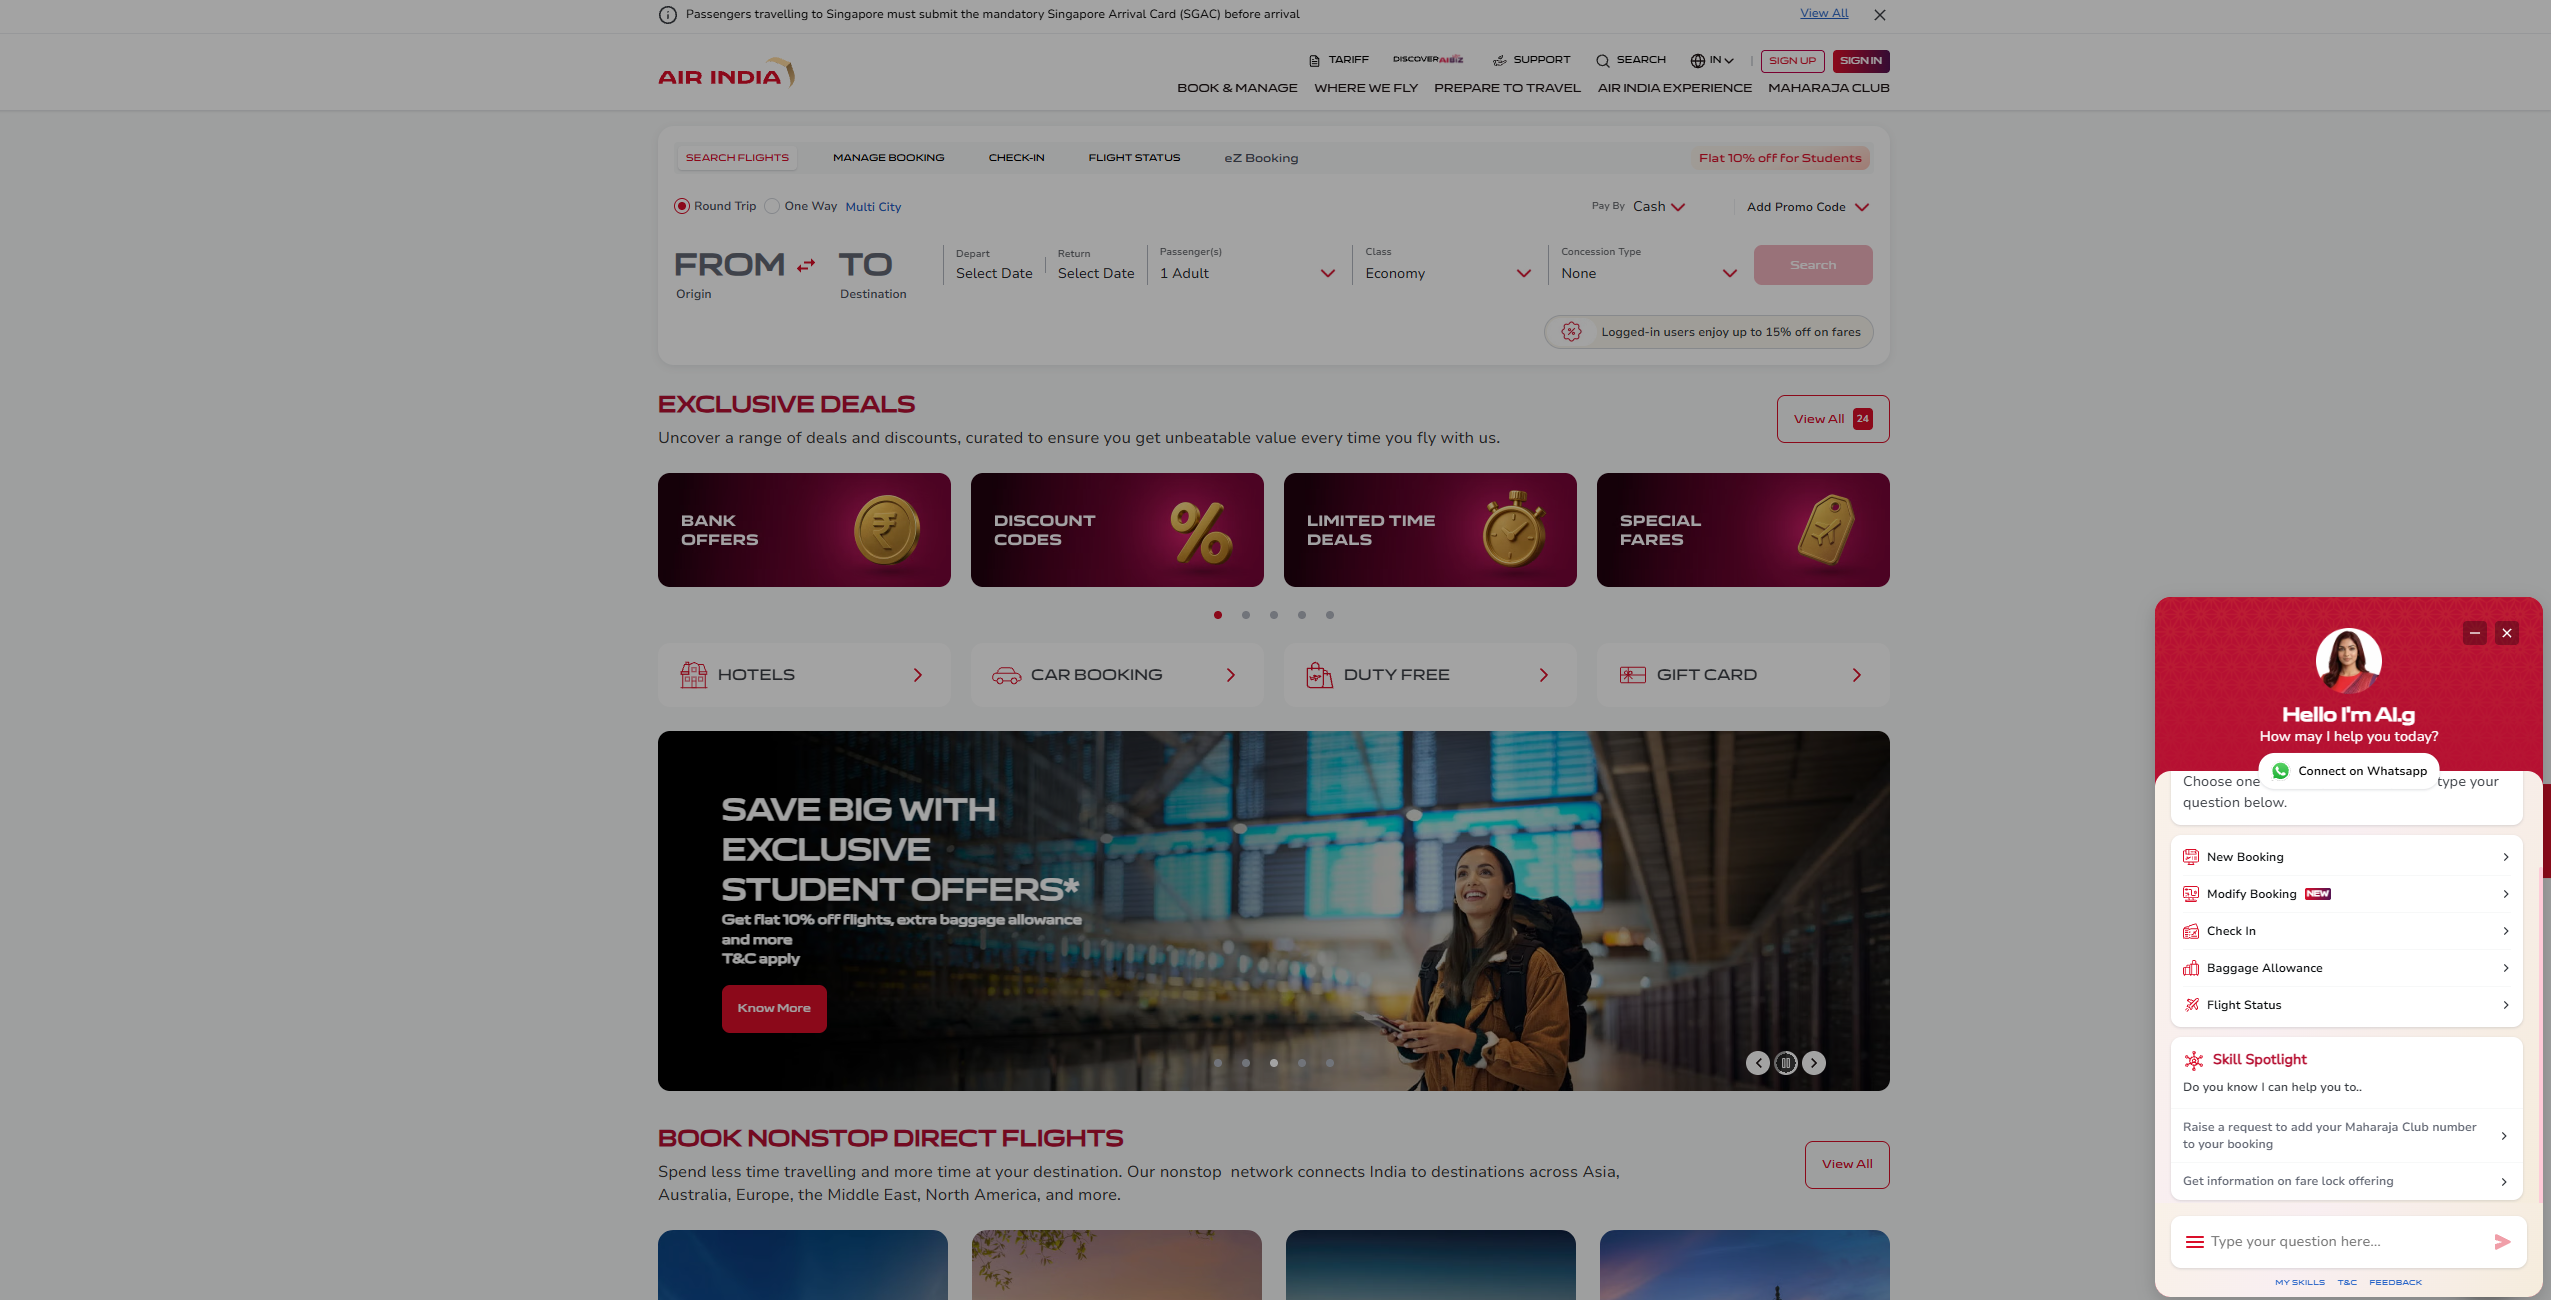
\includegraphics[width=0.98\linewidth]{given_UI_example.png}

EXT-UI-002 Multiple device layout
EXT-UI-003 Multiple language support
EXT-UI-004 Feedback mechanism 
EXT-UI-004 Escalated chat redirect request to user
EXT-UI-005 Escalated chat window for university side to answer questions
EXT-UI-006 Knowledge manager window
EXT-UI-007 History (Open questions)?


\subsection{Hardware Interfaces}
Because \textbf{FYNDR AI} is a web-based software application, it does not interface directly with custom physical hardware sensors or actuators. Instead, it relies on standard client and server hardware abstractions provided by the operating environment.

EXT-HW-001 website works on device (phone, laptop, desktop, MACOS, etc.)
EXT-HW-002 Server Hosting (local or cloud| open questions)?


\subsection{Software Interfaces}
This subsection specifies the interfaces between FYNDR AI and external software systems, browsers,
databases, AI inference services, and authentication providers.

EXT-SW-001 the website must embedd the chatbot
EXT-SW-002 the chatbot must interface with an online search engine for whitelisted sources
EXT-SW-003 the chatbot must interface with a local search engine for whitelisted sources
EXT-SW-004 the chatbot must interface with an LLM 
EXT-SW-005 the LLM the chatbot is connected with must be restricted harshly
EXT-SW-006 the management options must be restricted to a login with university credentials
EXT-SW-007 the chatbot must interface with a scraper/crawler to redirect the user directly to the information they want

\subsection{Communications Interfaces}
This subsection defines the network protocols, API formats, and external communication channels required by FYNDR AI.

EXT-COM-001 Encryption?
EXT-COM-002 Frontend - Backend communication
EXT-COM-003 Restricted internet access
EXT-COM-004 open/read to escalation chat

% ------------------------------------------------------------------------------
\section{System Features}
% ------------------------------------------------------------------------------
\guidance{Organize the functional requirements for the product by system features or use cases. Copy subsection 4.1 for each additional feature.}

\subsection{User Authentication and Profile Management}
\subsubsection{Description and Priority}
This feature allows DHBW students and lecturers to securely log into the platform using their university credentials and manage their profile settings. \textbf{Priority: High} (Benefit: 9, Penalty: 8, Cost: 3, Risk: 2).

\subsubsection{Stimulus/Response Sequences}
\begin{enumerate}
    \item \textbf{Stimulus:} User clicks ``Login with DHBW Account'' on the landing page.
    \item \textbf{Response:} System redirects to the university authentication provider.
    \item \textbf{Stimulus:} User enters valid credentials and confirms.
    \item \textbf{Response:} System creates a user session and displays the personal dashboard.
\end{enumerate}

\subsubsection{Functional Requirements}
% Example for using the requirements macro
\req{FR-01}{DHBW Single Sign-On}{High}{
    The system shall allow users to authenticate using their official DHBW university credentials. If authentication fails, an informative error message shall be displayed without revealing sensitive account details.
}

\req{FR-02}{Role Assignment}{High}{
    Upon first successful login, the system shall automatically assign the user role (Student or Lecturer) based on the directory attributes returned by the identity provider (see \reqref{FR-01}).
}

\subsection{System Feature 2 (Replace with Feature Name)}
\subsubsection{Description and Priority}
\guidance{Provide a short description of the feature and indicate whether it is of High, Medium, or Low priority.}

\subsubsection{Stimulus/Response Sequences}
\guidance{List the sequences of user actions and system responses that stimulate the behavior defined for this feature.}

\subsubsection{Functional Requirements}
\req{FR-03}{Example Requirement Title}{Medium}{
    The system shall ...
}

% ------------------------------------------------------------------------------
\section{Other Nonfunctional Requirements}
% ------------------------------------------------------------------------------

\subsection{Performance Requirements}
\req{NFR-01}{Page Load Response Time}{Medium}{
    95\% of all user interactions and page requests shall complete within 1.5 seconds under a simulated load of 100 concurrent campus users.
}

\subsection{Safety Requirements}
\guidance{Specify those requirements that are concerned with possible loss, damage, or harm that could result from the use of the product.}

\subsection{Security Requirements}
\req{NFR-02}{Transport Encryption}{High}{
    All network communication between client browsers and the backend server shall be encrypted using TLS 1.3 or higher.
}

\subsection{Software Quality Attributes}
\guidance{Specify additional quality characteristics such as adaptability, availability, maintainability, reliability, and usability.}

\subsection{Business Rules}
\guidance{List any operating principles about the product, such as which individuals or roles can perform which functions under specific circumstances.}

% ------------------------------------------------------------------------------
\section{Other Requirements}
% ------------------------------------------------------------------------------
\guidance{Define any other requirements not covered elsewhere in the SRS (e.g., database persistence requirements, GDPR/DSGVO compliance, internationalization).}

% ------------------------------------------------------------------------------
% Appendix
% ------------------------------------------------------------------------------
\newpage
\appendix
\renewcommand{\thesection}{Appendix \Alph{section}:}
\titleformat{\section}{\normalfont\Large\bfseries}{\thesection}{0.5em}{}

\section{Glossary}
\guidance{Define all the terms necessary to properly interpret the SRS, including acronyms and abbreviations.}
\begin{description}
    \item[DHBW] Duale Hochschule Baden-Württemberg.
    \item[SRS] Software Requirements Specification.
    \item[TBD] To Be Determined.
\end{description}

\section{Analysis Models}
\guidance{Include any pertinent analysis models, such as use-case diagrams, data flow diagrams, class diagrams, or entity-relationship diagrams.}

\section{To Be Determined List}
\guidance{Collect a numbered list of the TBD references that remain in the SRS so they can be tracked to closure.}
\begin{enumerate}
    \item \textbf{TBD-01:} Clarify with customer team whether offline caching is required for mobile devices (refers to Section 2.4).
\end{enumerate}

\end{document}
```
### Fully AI-generated template using Gemini based on the provided document
### How to get the most out of it in inscrive:
2. **Manage & link requirements:** With the `\req{ID}{Title}{Priority}{Text}` command, each requirement is displayed in a uniform box and automatically registered as a jump target. Anywhere in the document, you can then simply write `\reqref{FR-01}` to create a clickable reference in the PDF.
3. **Remove guidance text:** All italicized `<...>` notes from the original template are included via the `\guidance{...}` macro – simply replace them step by step with your own text.